\documentclass[a4paper,ngerman]{scrartcl}

\usepackage{amsmath}
\usepackage{amsfonts}
\usepackage{amssymb}
\usepackage[utf8]{inputenc}
\usepackage{graphicx}
\usepackage[ngerman]{babel}
\usepackage{hyperref}
\usepackage{float}
\usepackage{caption}
\usepackage{subcaption}
\usepackage{multirow}  %for tables
\usepackage{icomma} % Handle german comma as decimal point in numbers
\usepackage{units,siunitx} % Write units with correct spacing
\usepackage{upgreek} % provide non-italic greek letters
\usepackage{url}
%\usepackage{subfig}

% Formatting of table & figure captions
\captionsetup{font={sf,footnotesize},labelfont=bf,skip=6pt}
\setlength{\abovecaptionskip}{6pt}
\setlength{\belowcaptionskip}{0pt}

\title{Quantenradierer}
\date{\today}
\author{Michel Rausch, Michael Eliachevitch}

%\renewcommand\thesection{A\arabic{section}:\ }

\begin{document}

\maketitle
\tableofcontents
\clearpage

\section{Aufbau des Mach-Zehnder-Interferometers}
\label{sec:aufbau}
Das Mach-Zehnder-Interferometer wurde wie in Kapitel 4.1 der Versuchsvorbereitung beschrieben aufgebaut. 
Am aufwendigsten war es, die beiden Teilstrahlen mithilfe des Beamwalks zur Interferenz zu bringen.
Der erste Strahlteiler und der Spiegel von einem der beiden Teilstrahlen wurden fest gewählt, während 
der zweite Strahlteiler und der Spiegel von dem anderen Strahlteiler variiert wurden, um diesen zweiten Teilstrahl 
mit dem ersten Teilstrahl zur Interferenz zu bringen. Als Referenpunkte wurden die Positionen der Teilstrahlen 
auf dem ersten Strahlteiler und die Punkte auf dem Schirm gewählt. Für die Justierung haben wir die Wand als Schirm verwendet,
da sie weiter weg ist und daher bei gleichem Winkel größere Ablenkungen zustande kommen.\\

Der Aufbau war sehr störanfällig. Als wir bereits Interferenz hatten, wurde durch eine versehentliche Berührung eines der Spiegel 
die Interferenz wieder zerstört und wir mussten erneut den Beam Walk durchführen. Bei vorhandener Interfenz sah das Schirmbild wie 
in Abbildung \ref{fig:interferenz} dargestellt aus.

\begin{figure}[tbh!]
  \centering
  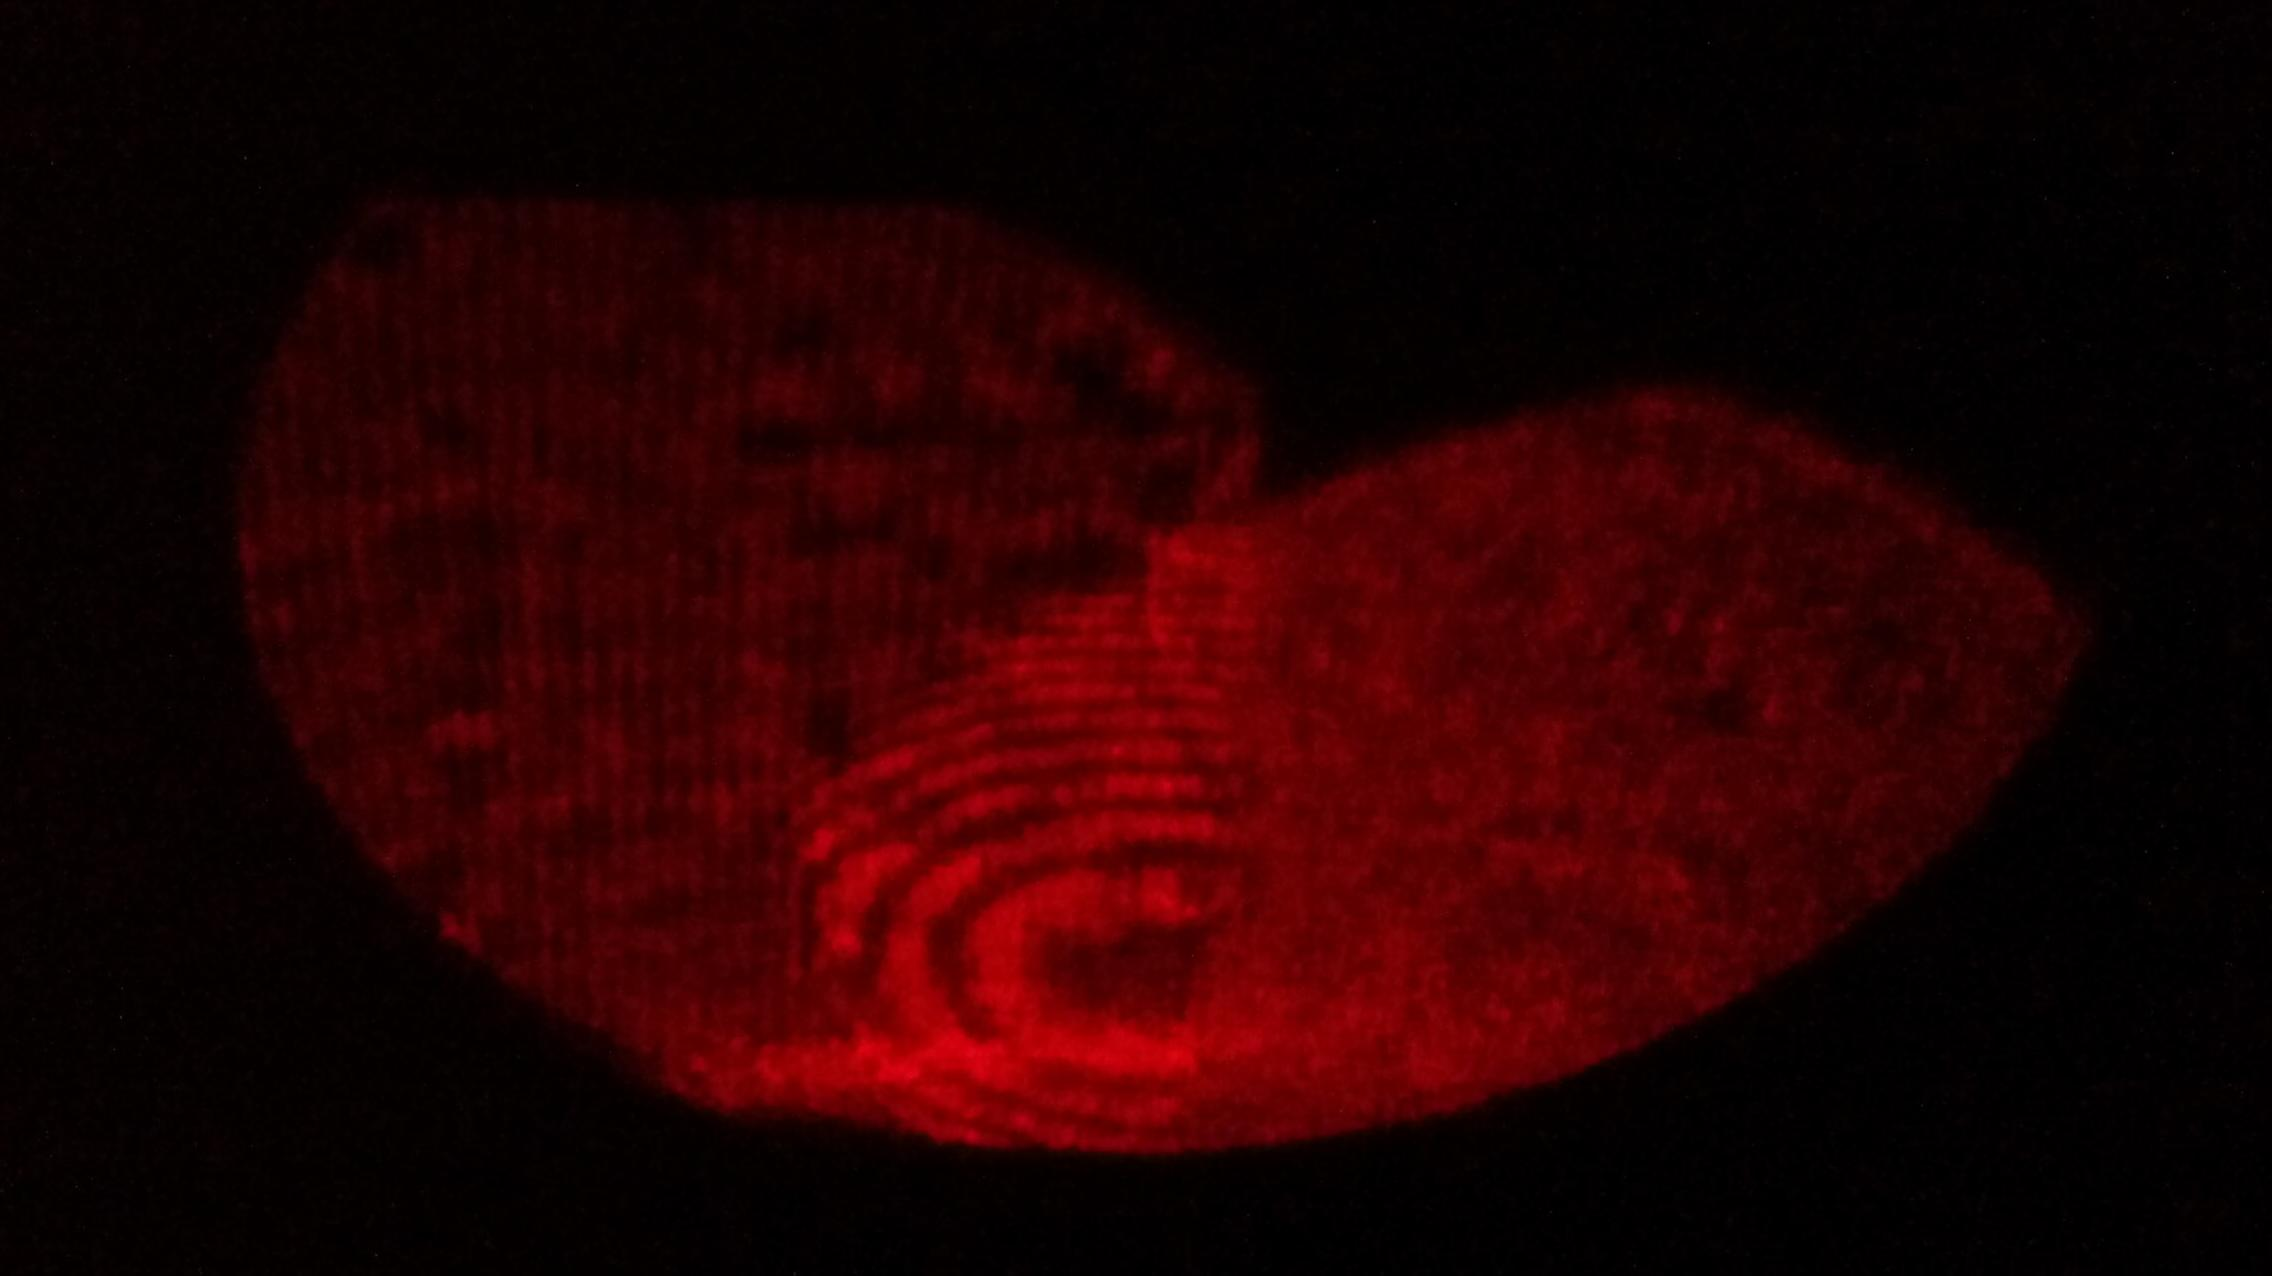
\includegraphics[width=0.5\textwidth]{fotos/interferenz_zugeschnitten.jpg}
  \caption{Schirmbild des Mach-Zehnder-Interferometers bei vorhandener Interferenz. Die "`Welcher-Weg-Information"' wurde dem Strahl hier nicht mitgegeben. Die konzentrischen Ringe entstehen aufgrund der Phasenunterschiede, die abhängig vom Strahlparameter an der Divergenz an den Linsen zustandekommen.}
  \label{fig:interferenz}
\end{figure}

\section{Anbringen der Polarisatoren}
Anschließend wurden wie in der Vorbereitung beschrieben an einem der Teilstrahl ein Polarisator im Winkel von 45\,Grad und am anderen 
ein Polarisator im Winkel von -45\,Grad angebracht, sodass die beiden Teilstrahlen danach orthogonal polarisiert waren.
Das war deswegen schwierig, da die Winkelangaben an den Polarisatoren nicht korrekt waren und daher nur als relative Winkel zu verstehen waren.
Um sie nun richtig einzustellen, wurden beide Polarisatoren jeweils so lange gedreht, bis sie senkrecht zu einem Referenzpolarisator vor
dem Laser waren, was an einem Minimum der Laseintensität hinter den Polarisatoren zu sehen war. So hatten beide Polarisatoren jeweils einen absoluten Winkel von 90\,Grad. Aus dieser Position wurden sie nun 45 Grad in unterschiedliche Richtungen gedreht. Sicherheitshalber wurde noch geprüft, ob sie auch orthogonal zueinander sind. Hintereinandergestellt blockierten sie den Laserstrahl, was für eine richtige Justierung sprach.\\

Wenn man die Polarisatoren nun an die Teilstrahlen anbrachte, verschwand das Interferenzmuster, wie in Abbildung \ref{fig:keine_interferenz} zu 
sehen ist. Das entspricht unserer Erwartung, da im Wellenbild der Interferenzterm verschwindet und quantemechanisch eine "`Welcher-Weg-Information"' mitgegeben wurde, sodass die Wellenfunktion der Teilchen nicht alle Wege berücksichtigen konnte. Durch die 
Anbringung der Polarisatoren hatten wir die Wellenfunktion also zum Kollaps gebracht.

\begin{figure}[tbh!]
  \centering
  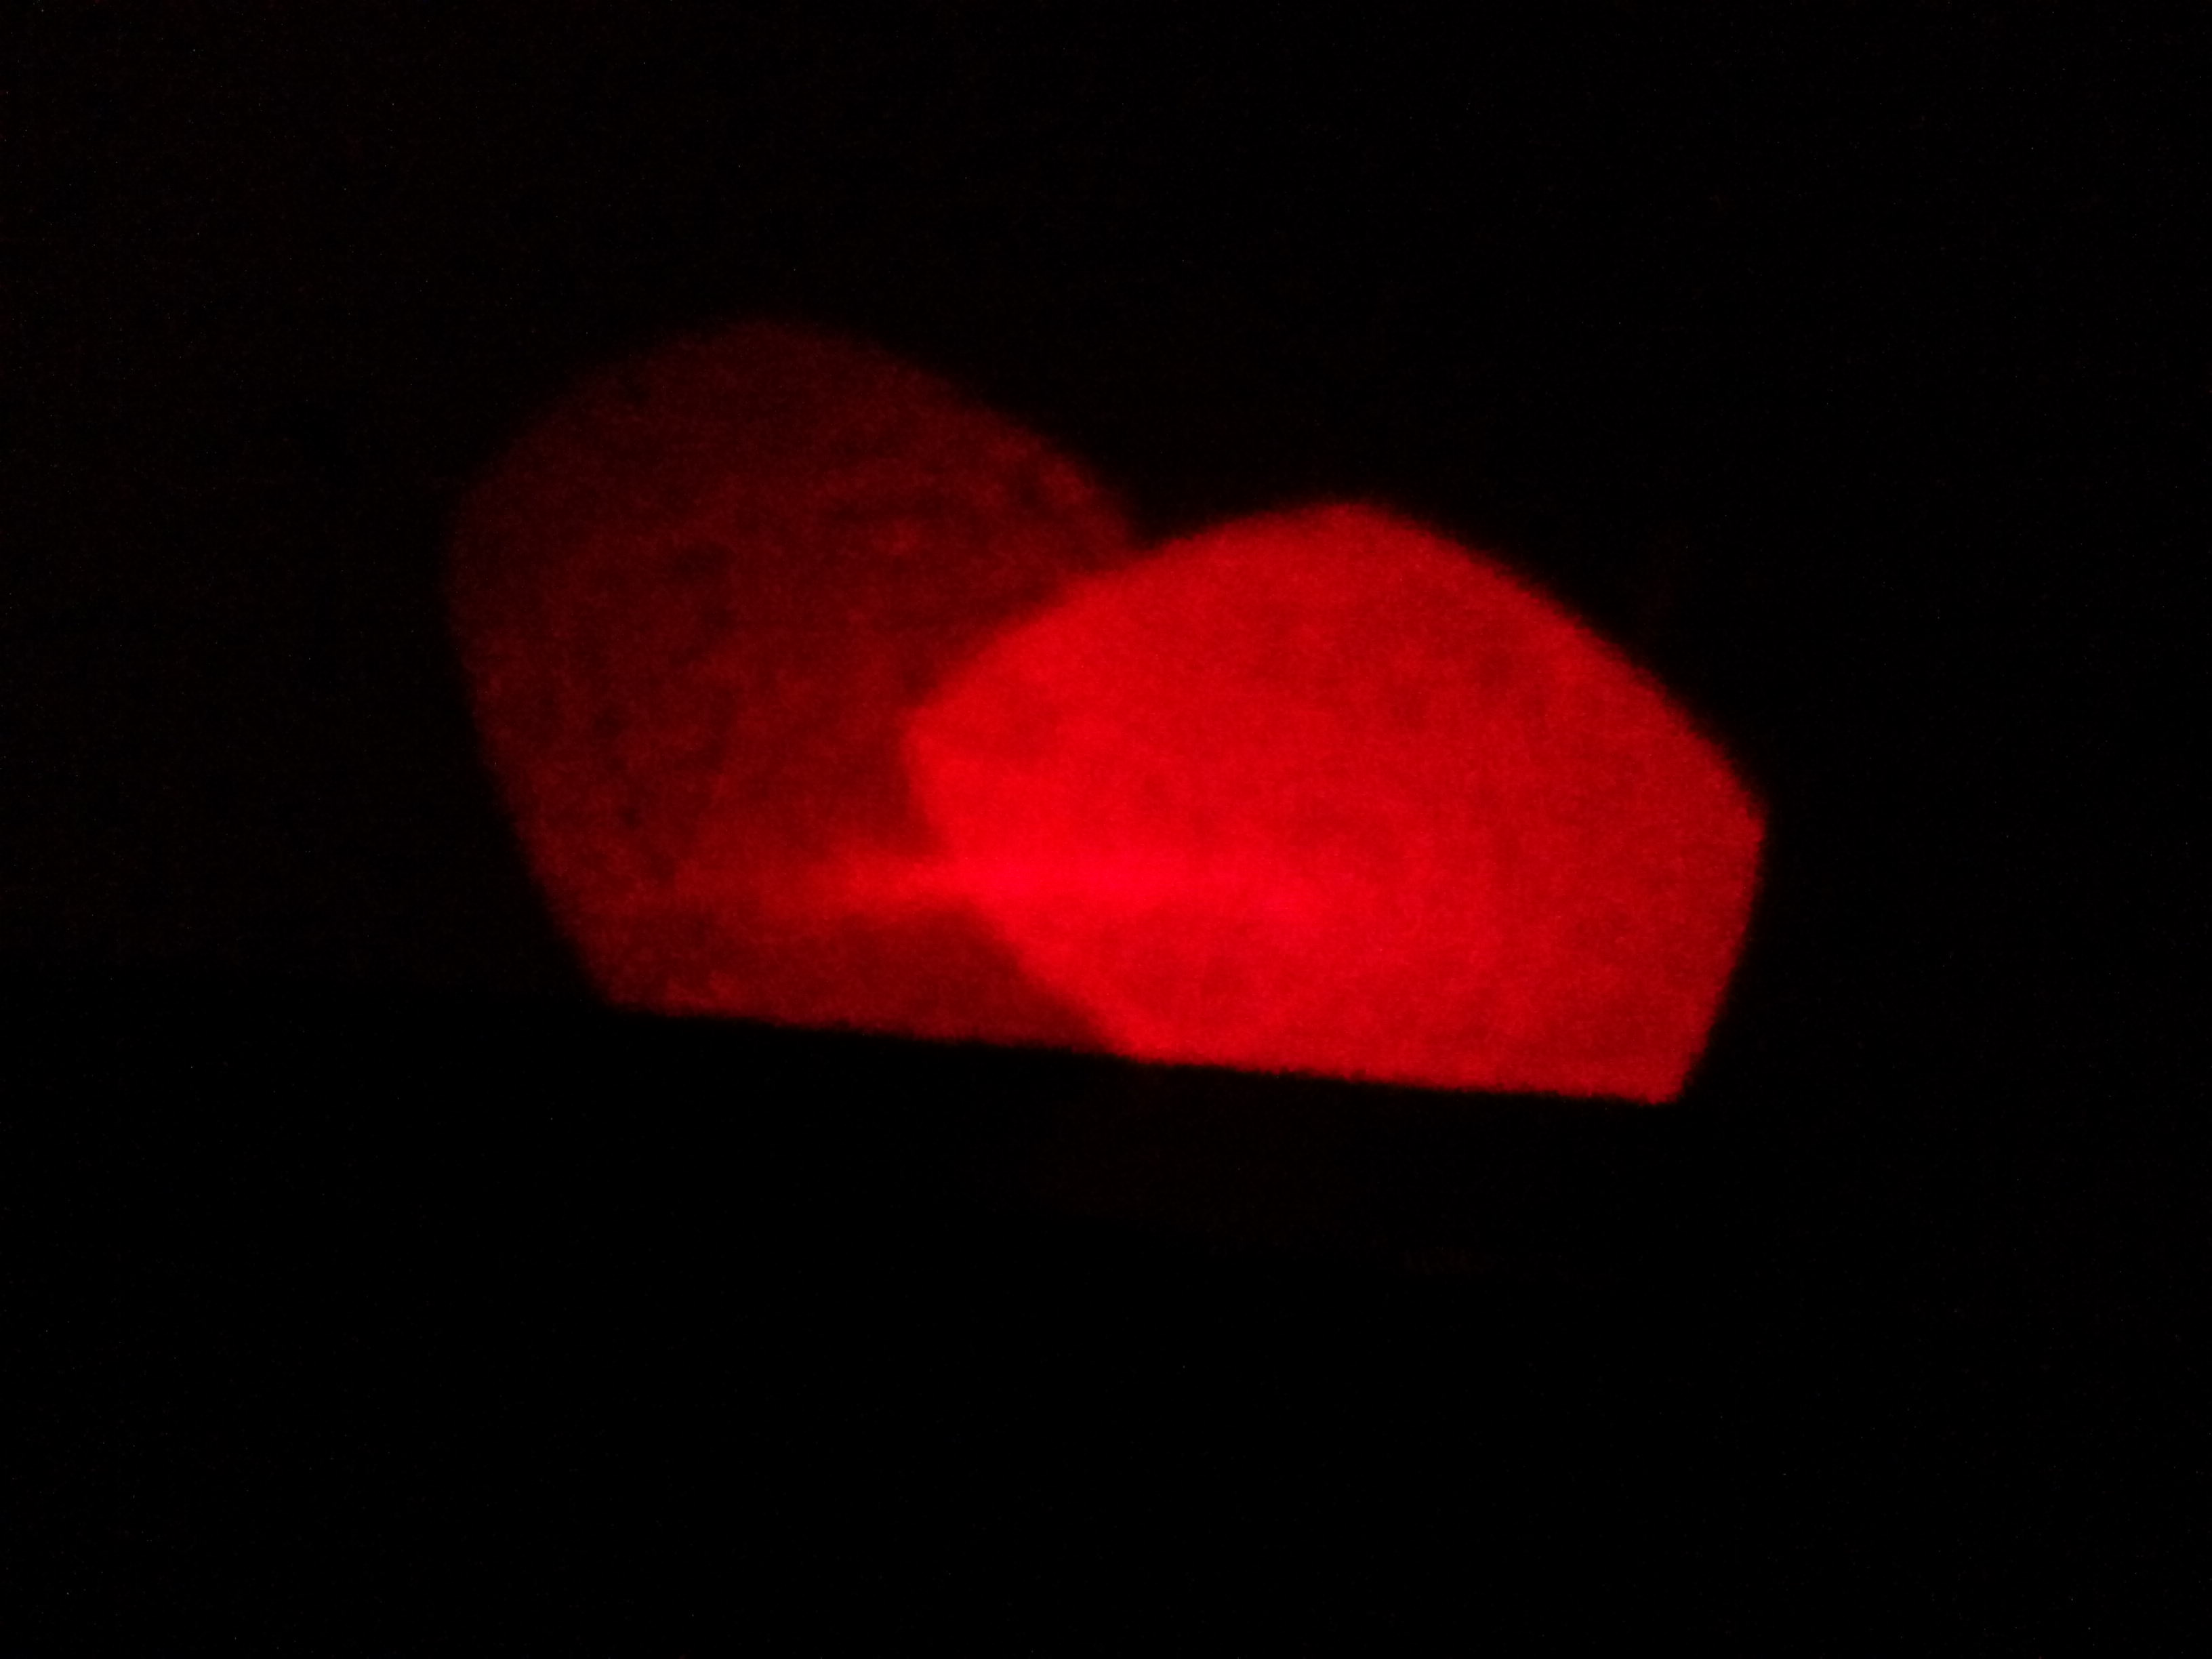
\includegraphics[width=0.5\textwidth]{fotos/ohne_qr_keineinterferenz.jpg}
  \caption{Schirmbild des Mach-Zehnder-Interferometers bei nicht vorhandener Interferenz. Die "`Welcher-Weg-Information"' wurde dem Strahl hier durch das Anbringen von einem Polarisator an jeweils jedem der beiden Teilstrahlen mitgegeben, wobei die Polarisatoren zueinander orthogonal waren. Im Wellenbild kann das Verschwinden des Interferenzbildes damit erklärt werden, dass durch die orthogonale Polarisation der Interferenzterm verschwindet. Quantenmechanisch kann man sagen, dass weil die Teilchen eine Information mit sich tragen, welchen Weg sie "`gegangen"' sind, sie nicht alle Wege gehen können und dadurch nicht mit sich selbst interferieren können. In der Quantenmechanik sagt man auch, dass durch die "`Messung"' des Weges
die Wellenfunktion der Teilchen kollabiert ist.}
  \label{fig:keine_interferenz}
\end{figure}

\section{Anbringen des Quantenradierers}
Zuletzt haben wir noch vor dem Schirm einen dritten Polarisator in einem absoluten Winkel von 0\,Grad angebracht. 
Dadurch war wieder ein Interferenzmuster zu sehen, ähnlich wie in Abbildung \ref{fig:interferenz} zu dargestellt ist. Auch das entsprach unseren Erwartungen. Denn durch den dritten Polarisator wurden die Polarisationen der beiden Teilstrahlen wieder identisch, wodurch sie ununterscheidbar wurden.
Die "`Welcher-Weg-Information"' wurde also wieder gelöscht und die Wellenfunktion jedes Teilchens konnte nun wieder alle Wege zum Schirm berücksichtigen. Dieser dritte Polarisator war somit ein Beispiel eines sogenannten Quantenradierers. Auch im klassischen Wellenbild 
ist die Wiederherstellung des Interfenzmuster erklärbar. Durch den dritten Polarisator wurden beide Teilstrahlen gedreht, sodass sie wieder diesselbe Polarisation hatten und wieder miteinander interferieren konnten, der Interferenzterm tauchte wieder auf.

\section{Gedankenexperiment: Einphotonenlaser}
Wenn man das selbe Experiment mit einzelnen Photonen durchführen würde, könnte man die Möglichkeit ausschließen, dass die Photonen im Laser
untereinander wechselwirken. Wenn man durch das Interferometer oft genug einzelne Photonen schicken würde, wäre gemittelt über einen 
längeren Zeitraum zu erwarten, das wieder dasselbe Interferenzmuster auftaucht. Das liegt daran, dass die Wellenfunktion jedes einzelnen Teilchens immer alle möglichen Wege zu einem bestimmten Punkt auf dem Schirm berücksichtigt. In der klassischen Physik macht es keinen Sinn, von einzelnen Photonen zu reden, da sie die Quantelung von Energie in Photonen nicht berücksichtigt. Dennoch ist jedes Photon eine Anregung des elektromagnetischen Feldes, selbst bei einzelnen Photonen, und daher hat man auch bei einzelnen Photonen eine elektromagnetische Welle, die beide Wege geht und mit sich selbst interferiert.





\end{document}
